\section{Data reviewing}
\subsection{Data description}
\hspace{\parindent}
The data is from Kaggle. Below is description about the dataset\\

\begin{table}[H]
	\begin{tabular}{|p{3cm}|p{2cm}|p{10cm}|}
		\hline
		\textbf{Attribute} & \textbf{Type} &  \textbf{Description} \\
		\hline
		Step & Numerical & Shows a chunk of time, where each step means one hour. \\
		Type & Categorical & Tells what kind of online action it is. \\
		Amount & Numerical & How much money is being moved in the transaction. \\
		NameOrig & Text & The person who starts the transaction. \\
		OldbalanceOrg & Numerical & The amount of money they had before. \\
		NewbalanceOrig & Numerical & The amount they have after. \\
		NameDest & The Text & person getting the money. \\
		OldbalanceDest & Numerical &How much they had before. \\
		NewbalanceDest & Numerical & How much they have after. \\
		IsFraud & Binary & Says if the transaction is a scam or not. \\
		isFlaggedFraud & Binary & Indicator flagging potentially fraudulent transactions based on specific criteria. \\
		\hline
	\end{tabular}
	\caption{Data description}
	\label{tab:Functional}
\end{table}


\subsection{Check unique values}

\begin{figure}[H]
	\centering
	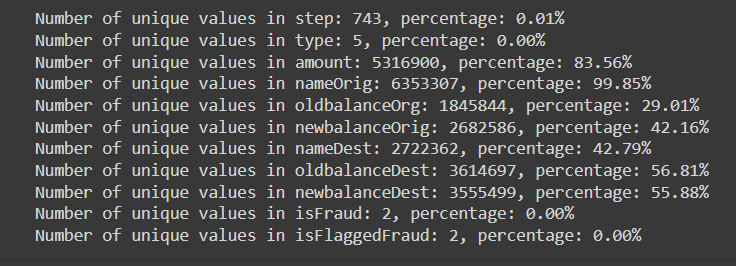
\includegraphics[width=0.7\linewidth]{chap4/unique_values}
	\caption{Unique Values}
	\label{fig:uniquevalues}
\end{figure}

\begin{itemize}
	\item Step: The 'step' column has 743 unique values, which seems reasonable if it represents a discrete time step. The percentage of unique values is extremely low (0.0117\%), indicating that the 'step' values are quite distributed or densely packed.
	\item Type: The 'type' column has 5 unique values, which could represent different types of financial transactions. The percentage of unique values is very low (7.86e-05\%), indicating that the 'type' values are relatively evenly distributed.
	\item Amount: The 'amount' column has a large number of unique values (5,316,900), which is expected as it represents the monetary amount of transactions. The percentage of unique values is high (83.56\%), suggesting a wide range of transaction amounts.
	\item NameOrig: The 'nameOrig' column has a very high number of unique values (6,353,307), which indicates that each transaction initiator has a unique identifier. The percentage of unique values is almost 100\%, suggesting almost every transaction initiator has a unique identifier.
	\item OldbalanceOrg, NewbalanceOrig, NameDest, OldbalanceDest, NewbalanceDest: These columns all have a significant number of unique values, suggesting diversity in account balances and destination names. The percentages of unique values range from 29\% to 56\%, indicating moderate to high diversity in these columns.
	\item IsFraud, IsFlaggedFraud: These binary columns have only 2 unique values each, which is expected for binary indicators. The percentages of unique values are extremely low (0.0000314\%), indicating that the overwhelming majority of transactions are non-fraudulent and not flagged as fraud.
\end{itemize}

\subsection{Check missing values}

\begin{figure}[H]
	\centering
	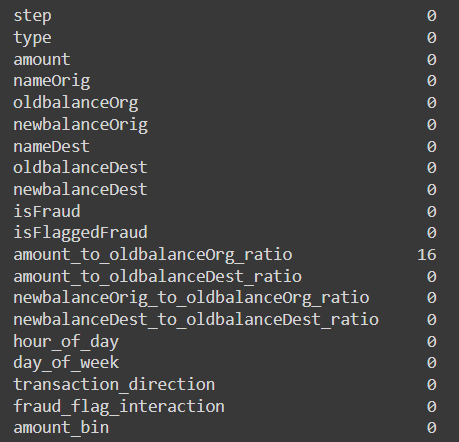
\includegraphics[width=0.7\linewidth]{chap4/missing_values}
	\caption{Missing Values}
	\label{fig:missingvalues}
\end{figure}

The dataset seems to be well-prepared, with most columns having no missing values. However, the presence of missing values in the 'amount\_to\_oldbalanceOrg\_ratio' column suggests potential data issues in that specific calculation or input data.\\


\section{Data visualization}

\begin{figure}[H]
	\centering
	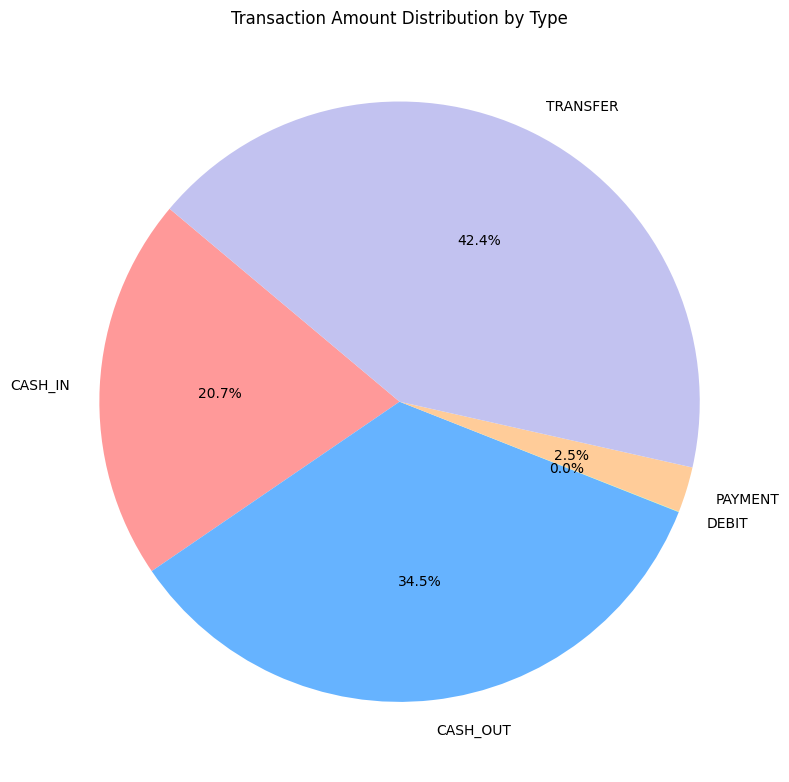
\includegraphics[width=0.7\linewidth]{chap4/1}
	\caption{Transfers and cash-outs as dominant contributors, representing 42.4\% and 34.5\% of the total transaction amount respectively. Payments constitute a smaller portion at 2.5\%, while debit transactions have minimal impact. Cash-ins also play a notable role, contributing 20.7\% to the overall transaction volume}
	\label{fig:1}
\end{figure}

\begin{figure}[H]
	\centering
	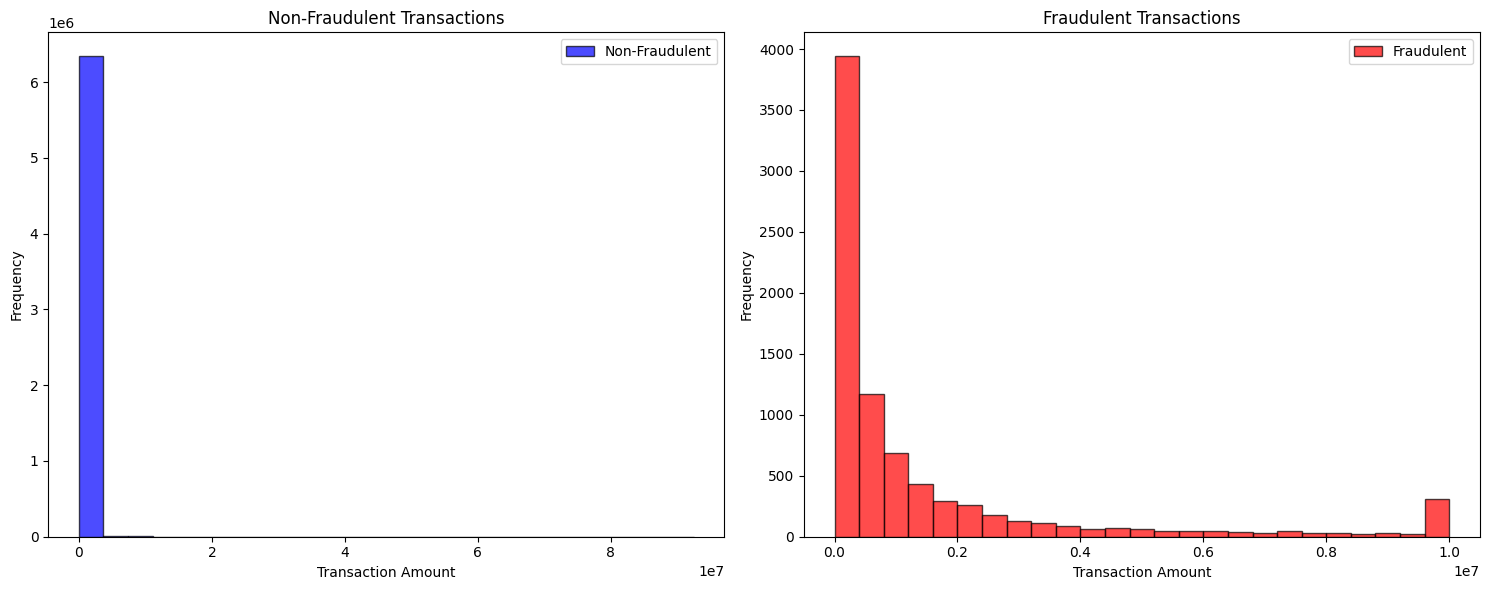
\includegraphics[width=0.7\linewidth]{chap4/2}
	\caption{Comparison of the distribution of transaction amounts between fraudulent and non-fraudulent transactions, aiding in understanding patterns and differences in transaction behavior}
	\label{fig:2}
\end{figure}

\begin{figure}[H]
	\centering
	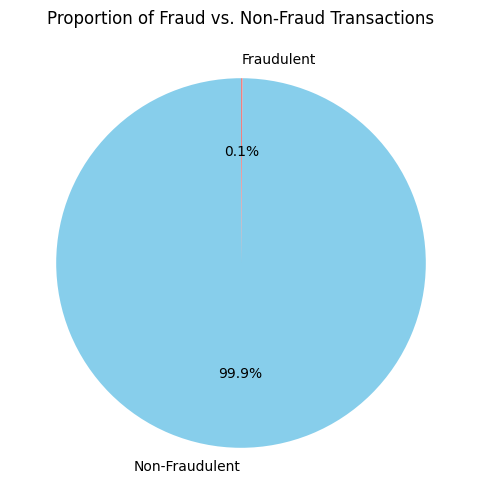
\includegraphics[width=0.7\linewidth]{chap4/3}
	\caption{Proportion of Fraud vs. Non-Fraud Transactions}
	\label{fig:3}
\end{figure}

\begin{figure}[H]
	\centering
	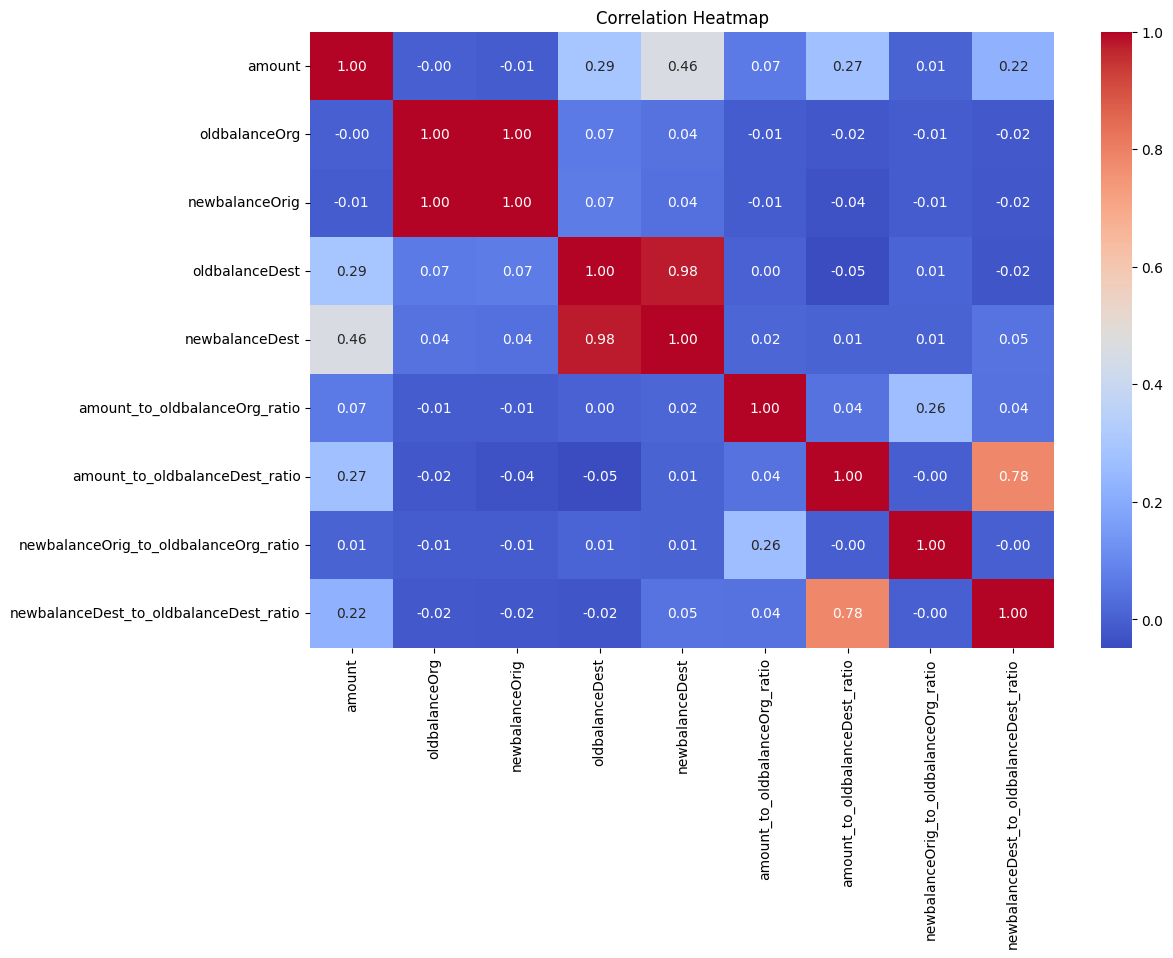
\includegraphics[width=0.7\linewidth]{chap4/4}
	\caption{The correlation between numerical features in the dataset, with warmer colors indicating stronger positive correlations and cooler colors representing stronger negative correlations. Values closer to 1 or -1 signify higher correlation, while values closer to 0 indicate weaker correlation. This visualization aids in identifying potential relationships and dependencies between different variables in the dataset}
	\label{fig:4}
\end{figure}



\section{Data preprocessing}
\subsection{Remove null values}
\hspace{\parindent}
The dataset contained null values in one feature, namely \texttt{amount\_to\_oldbalanceOrg\_ratio}. To address this issue, a common approach of filling null values with the mean of the column was employed.


\subsection{Determine transaction direction}
\hspace{\parindent}
A new feature, \texttt{transaction\_direction}, was created to categorize transactions as either outgoing or incoming based on the transaction amount. This binary categorization enhances the dataset by providing insights into the nature of each transaction. Outgoing transactions are labeled as 'Outgoing' if the amount is greater than zero, and 'Incoming' otherwise.

\subsection{Create amount bins}
\hspace{\parindent}
The continuous variable \texttt{amount} was discretized into bins to simplify its representation and potentially capture nonlinear relationships between transaction amounts and other features. The following bins were defined:

\begin{itemize}
	\item Very Low: Amounts between $0$ and $1000$
	\item Low: Amounts between $1000$ and $5000$
	\item Medium: Amounts between $5000$ and $10000$
	\item High: Amounts between $10000$ and $50000$
	\item Very High: Amounts above $50000$
\end{itemize}

These bins were created using the \texttt{cut} function from the \texttt{pandas} library in Python. The resulting discrete variable, \texttt{amount\_bin}, allows for a more straightforward analysis of the transaction amounts and their potential impact on fraud detection.



\subsection{Encode categorical features}
\hspace{\parindent}
Categorical features such as \texttt{nameOrig}, \texttt{nameDest}, \texttt{transaction\_direction}, and \texttt{amount\_bin} were encoded using the LabelEncoder from the scikit-learn library. This preprocessing step converts categorical variables into numerical labels, facilitating their use in machine learning models.


\subsection{Construct Node Features and Edges}
\hspace{\parindent}
Node features and edges were constructed for the graph representation using the provided data. Node features were derived from selected attributes including 'amount', 'oldbalanceOrg', 'newbalanceOrig', 'oldbalanceDest', and 'newbalanceDest', and converted into a torch tensor of type \texttt{float32}.


\begin{tikzpicture}[
	node/.style={draw, circle, minimum size=1cm},
	edge/.style={->, >=Stealth}
	]
	% Nodes
	\node[node] (n1) {$x_1$};
	\node[node, below=1.5cm of n1] (n2) {$x_2$};
	\node[node, below=1.5cm of n2] (n3) {$x_3$};
	
	% Node features
	\node[right=2cm of n3, align=center] (features) {Node Features: \\ 'amount', 'oldbalanceOrg', \\ 'newbalanceOrig', 'oldbalanceDest', \\ 'newbalanceDest'};
	
	% Edges
	\draw[edge] (n1) -- (n2);
	\draw[edge] (n2) -- (n3);
	\draw[edge] (n1.east) -- (features.west);
	\draw[edge] (n2.east) -- (features.west);
	\draw[edge] (n3.east) -- (features.west);
\end{tikzpicture}

To establish unique identifiers for nodes, a mapping was created based on the 'node\_identifier' column, ensuring each node has a distinct identifier. The 'nameOrig' and 'nameDest' columns were updated accordingly using the generated mapping.

Edges were defined using the 'nameOrig' and 'nameDest' columns, and converted into a torch tensor of type \texttt{long}, ensuring compatibility with PyTorch. The resulting data structure, \texttt{data}, encapsulates both node features and edge information, facilitating subsequent graph neural network operations.

\begin{figure}[H]
	\centering
	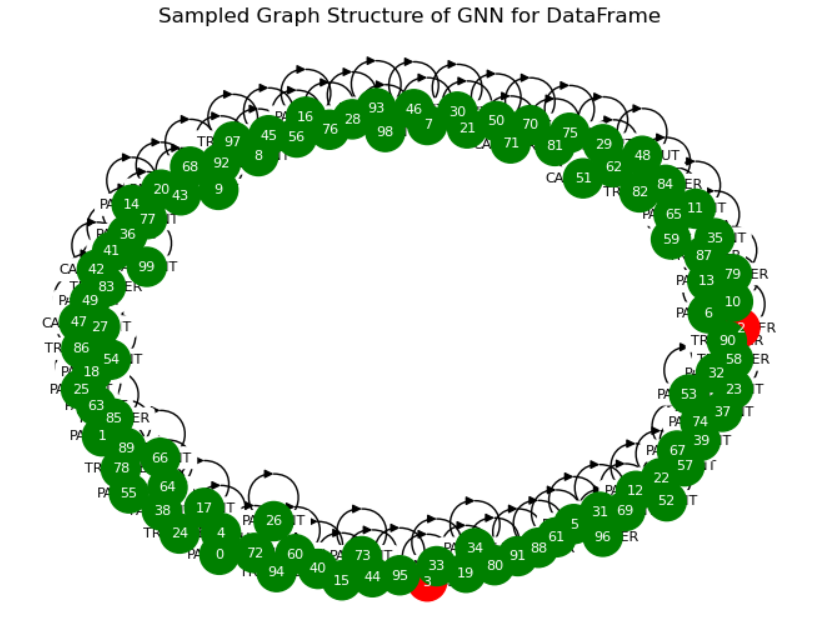
\includegraphics[width=0.7\linewidth]{chap4/5}
	\caption{Visualize the GNN}
	\label{fig:5}
\end{figure}


\section{Graph Neural Network Architecture}
\hspace{\parindent}
The graph neural network (GNN) architecture used for fraud detection in online payments comprises multiple layers of graph convolutional units, each processing information from neighboring nodes within the payment network.

The GNN model consists of two graph convolutional layers (\texttt{GCNConv}), with the first layer transforming input node features to a hidden representation and the second layer further refining the hidden representation to produce the final output.

The \texttt{forward} method of the \texttt{GNNModel} class defines the forward pass of the model. It takes the input graph data, including node features (\texttt{x}) and edge indices (\texttt{edge\_index}), and applies the graph convolutional layers to propagate information through the graph. The ReLU activation function is applied after each convolutional layer to introduce non-linearity to the model.

This architecture leverages graph convolutional operations to capture complex relationships and patterns within the online payment network, enabling effective fraud detection through graph-based learning mechanisms.

\begin{figure}[H]
	\centering
	\resizebox{\textwidth}{!}{%
		\begin{tikzpicture}[
			node/.style={draw, circle, minimum size=1cm},
			layer/.style={draw, rectangle, minimum width=2cm, minimum height=1cm},
			arrow/.style={->, >=Stealth}
			]
			% Input layer
			\node[node] (x1) {$x_1$};
			\node[node, below=0.5cm of x1] (x2) {$x_2$};
			\node[node, below=0.5cm of x2] (x3) {$x_3$};
			\node[node, below=0.5cm of x3] (x4) {$x_4$};
			\node[node, below=0.5cm of x4] (x5) {$x_5$};
			
			% Graph convolutional layers
			\node[layer, right=2cm of x3] (conv1) {Graph Convolutional Layer};
			\node[layer, right=2cm of conv1] (relu1) {ReLU Activation};
			\node[layer, right=2cm of relu1] (conv2) {Graph Convolutional Layer};
			
			% Output layer
			\node[node, right=2cm of conv2] (output) {Output};
			
			% Connections
			\foreach \i in {1,2,3,4,5}
			\draw[arrow] (x\i) -- (conv1);
			\draw[arrow] (conv1) -- (relu1);
			\draw[arrow] (relu1) -- (conv2);
			\draw[arrow] (conv2) -- (output);
		\end{tikzpicture}%
	}
	\caption{Graph Neural Network Architecture}
	\label{fig:gnn_architecture}
\end{figure}

\section{Training the Graph Neural Network}
\hspace{\parindent}
To train the Graph Neural Network (GNN) model for fraud detection in online payments, an optimizer and a loss criterion are defined. The optimizer, instantiated with the Adam optimizer from PyTorch, is utilized to update the parameters of the GNN model during training. Additionally, the CrossEntropyLoss function is employed as the loss criterion to compute the discrepancy between the model predictions and the ground truth labels.

The training process iterates over a fixed number of epochs, during which the optimizer is reset to zero gradients using the optimizer.zero\_grad() method. The output predictions of the GNN model (out) are computed using the forward pass with the input data (data). Subsequently, the loss between the predictions and the target labels is calculated using the defined loss criterion. The gradients are then backpropagated through the network using the loss.backward() method, and the optimizer updates the model parameters using the computed gradients with optimizer.step().

Following the training loop, the GNN model is evaluated on a held-out dataset to obtain node embeddings. The model is set to evaluation mode using gnn\_model.eval() to disable dropout and batch normalization layers that are active during training. Node embeddings are generated by applying the first graph convolutional layer (gnn\_model.conv1) to the input data (data.x) and edge indices (data.edge\_index). The resulting embeddings are detached from the computation graph using .detach() and converted to NumPy arrays for further analysis.


\begin{figure}[htbp]
	\centering
	\resizebox{\textwidth}{!}{%
		\begin{tikzpicture}[
			node/.style={draw, rectangle, minimum width=3.5cm, minimum height=0.75cm},
			process/.style={draw, rectangle, minimum width=4cm, minimum height=0.75cm, align=center},
			arrow/.style={->, >=Stealth}
			]
			% Nodes
			\node[process] (optimizer) {Optimizer: Adam};
			\node[process, below=0.5cm of optimizer] (criterion) {Loss Criterion: CrossEntropyLoss};
			\node[process, below=0.5cm of criterion] (loop) {Training Loop: 150 Epochs};
			
			% GNN model
			\node[process, right=3cm of criterion] (model) {GNN Model};
			\node[node, below=0.5cm of model] (data) {Input Data};
			\node[process, below=0.5cm of data] (forward) {Forward Pass};
			\node[process, below=0.5cm of forward] (loss) {Compute Loss};
			\node[process, below=0.5cm of loss] (backward) {Backward Pass};
			\node[process, below=0.5cm of backward] (update) {Update Parameters};
			
			% Evaluation
			\node[process, right=3cm of model] (evaluation) {Evaluation};
			\node[node, below=0.5cm of evaluation] (node_embeddings) {Node Embeddings};
			
			% Arrows
			\draw[arrow] (optimizer) -- (model);
			\draw[arrow] (criterion) -- (model);
			\draw[arrow] (loop) -- (model);
			\draw[arrow] (model) -- (data);
			\draw[arrow] (data) -- (forward);
			\draw[arrow] (forward) -- (loss);
			\draw[arrow] (loss) -- (backward);
			\draw[arrow] (backward) -- (update);
			\draw[arrow] (model) -- (evaluation);
			\draw[arrow] (evaluation) -- (node_embeddings);
		\end{tikzpicture}%
	}
	\caption{Training Process for the Graph Neural Network (GNN) Model}
	\label{fig:gnn_training_process}
\end{figure}

\section{Anomaly Detection and Fraud Identification}
\hspace{\parindent}
An Isolation Forest algorithm is utilized for anomaly detection to identify potentially fraudulent transactions within the online payment dataset. Initially, the Isolation Forest model is instantiated without any hyperparameters specified.

Subsequently, the Isolation Forest model is trained using the node embeddings obtained from the previously trained Graph Neural Network (GNN) model. These node embeddings serve as input features for the Isolation Forest algorithm.

Once the Isolation Forest model is trained, anomaly scores are computed for each transaction using the decision\_function() method. These anomaly scores indicate the degree of abnormality of each transaction within the dataset.

A threshold value is then set to classify transactions as potentially fraudulent or non-fraudulent based on their anomaly scores. Transactions with anomaly scores below the threshold are labeled as potentially fraudulent.

Finally, transactions identified as potentially fraudulent are printed to facilitate further investigation and analysis. This provides insights into suspicious transactions that may warrant additional scrutiny for potential fraudulent activity.

\begin{figure}[htbp]
	\centering
	\begin{tikzpicture}[
		node/.style={draw, rectangle, minimum width=3.5cm, minimum height=0.75cm},
		process/.style={draw, rectangle, minimum width=4cm, minimum height=0.75cm, align=center},
		arrow/.style={->, >=Stealth}
		]
		% Nodes
		\node[process] (iso_forest) {Isolation Forest};
		\node[process, below=0.5cm of iso_forest] (fit) {Fit Model};
		\node[process, below=0.5cm of fit] (decision) {Compute Anomaly Scores};
		\node[process, below=0.5cm of decision] (threshold) {Set Threshold};
		\node[process, below=0.5cm of threshold] (identify) {Identify Potentially Fraudulent Transactions};
		
		% Output
		\node[node, right=3cm of decision] (output) {Potentially Fraudulent Transactions};
		
		% Arrows
		\draw[arrow] (iso_forest) -- (fit);
		\draw[arrow] (fit) -- (decision);
		\draw[arrow] (decision) -- (threshold);
		\draw[arrow] (threshold) -- (identify);
		\draw[arrow] (identify) -- (output);
	\end{tikzpicture}
	\caption{Process of Anomaly Detection and Fraud Identification using the Isolation Forest Algorithm}
	\label{fig:anomaly_detection}
\end{figure}